\newpage
\pagenumbering{arabic}  %numero de pagina numeración arábiga
\setcounter{page}{1}    %comienza a contar desde 1

\chapter{Introducción}
\noindent La radiación incidente en los sensores es capaz de ionizar electrones del Si.  
La relación entre la carga producida y la energía incidente, es decir la energía necesaria para producir un par electrón-hueco resulta ser fundamental importancia para traducir espectros de carga en espectros de energía.

Por otro lado, existen diferentes fenómenos que modifican la forma de los espectros de carga producidos por la radiación incidente en los sensores. Entre ellos, los dos más importantes sonn: el factor de Fano, que cuantifica la dispersión de carga; y las deficiencias en la colección de carga, que tienden a producir colas a baja energía en los picos producidos por eventos monoenergéticos.

En este capítulo se describen estas tres cantidades, que constituyen propiedades del silicio y del sensor estudiadas en el marco de esta tesis, yendo mas allá del ruido de lectura gracias a la tecnología Skipper-CCD.

%%%%%%%%%%%%%%%%%%%%%%%%%%%%%%%%%%%%%%%%%%%%%%%%%%%%%%%%%%%%%%%%%%
%%%%%%%%%%%%%%%%%%%%%%%%%%%%%%%%%%%%%%%%%%%%%%%%%%%%%%%%%%%%%%%%%%
\section{Factor de Fano y energía de creación electrón-hueco}
\noindent El factor de Fano mide la relación entre la dispersión de una distribución de carga producida en un detector y su media. Viene dado por
\begin{equation*}
    F = \frac{\sigma^{2}}{\mu}
\end{equation*}
donde $\sigma^{2}$ es la varianza de la distribución de carga y $\mu$ es la media. 
Para el caso particular de una distribución de Poisson, la varianza y la esperanza coinciden, de forma que el factor de Fano equivale a $1$. 
Estas distribuciones de carga son el producto de la interacción de fotones de cierta energía con el detector, entre otros factores, que van depositando energía en el material ionizando cargas a su paso. 
\textcolor{red}{ASI PARECIERA QUE LOS FOTONES SON QUIENES IONIZAN A SU PASO, PERO EN REALIDAD SON LOS ELECTRONES QUE GANARON ENERGIA DE ESOS FOTONES, ARREGLAR.}

Dicha distribución tiene origen en que la energía transferida en cada interacción no es constante y, por lo tanto, para una dada energía inicial de la partícula incidente, tampoco será constante el número de cargas generadas.

Por otro lado, la energía de creación electrón-hueco $\varepsilon_{\eh}$ es medida en valor medio, ya que es calculada a través del cociente entre la energía entregada al detector y la carga en él producida. 
Además, se encuentra está relacionada con la energía del \textit{band gap} del silicio, entre la banda de valencia y la banda de conducción, que es $E_{g}\sim 1.1\,\si{eV}$\cite{Janesick}. Sin embargo, debido a que durante el proceso de interacción parte de la energía entregada al material puede disiparse emitiendo fonones, la energía de creación electrón-hueco resulta ser mayor, en promedio, que la energía del \textit{gap}.

La estimación precisa de ambas magnitudes es de vital importancia en la caracterización de este tipo de detectores, debido a que, por ejemplo, parámetros como la eficiencia cuántica dependen fuertemente de ellos. Además es importante determinar la dependencia de estas magnitudes con la energía ya que, en particular, el factor de Fano a energías por debajo de $1\,\si{keV}$ es clave para el cálculo de sensibilidad en experimentos de materia oscura liviana, como es caso del experimento SENSEI (\textit{Sub-Electron Noise Skipper-CCD Experiment Instrument})\cite{barak}.

%%%%%%%%%%%%%%%%%%%%%%%%%%%%%%%%%%%%%%%%%%%%%%%%%%%%%%%%%%%%%%%%%%
%%%%%%%%%%%%%%%%%%%%%%%%%%%%%%%%%%%%%%%%%%%%%%%%%%%%%%%%%%%%%%%%%%
\section{CCD y Skipper CCD}
\noindent Los dispositivos CCD (\textit{Charge Coupled Devices}) fueron inventados en 1969 en los Laboratorios Bell, por Willard Boyle y George Smith, en su búsqueda por fabricar dispositivos de memoria. Finalmente, los CCD's no fueron utilizados con este fin al ser superados por otras tecnologías, pero sí demostraron un gran potencial como sensores de luz y partículas. Tal es así que en el año 2010 sus inventores recibieron el premio Nobel de física\cite{Boyle, Smith}.

Estos dispositivos están hechos esencialmente de silicio y sus elementos constitutivos fundamentales son capacitores MOS (por \textit{metal-oxide-semiconductor}). Estos conforman los píxeles del detector, siendo por lo general millones y ocupando casi la totalidad de la superficie del sensor. Los capacitores MOS se componen generalmente de un sustrato semiconductor dopado, sobre el cual se deposita una delgada capa de óxido y a su vez sobre esta se coloca un metal de contacto. Este contacto metálico se encuentra a un voltaje $V_{G}$ y debajo del semiconductor se encuentra otro contacto que se encuentra a tierra. Dependiendo del valor de $V_{G}$ se obtienen distintos regímenes del MOS\cite{Chenming} donde, en particular, uno de ellos genera una región de depleción cerca del óxido, el cual permite acumular carga minoritaria.
\begin{figure}[h]
    \centering
        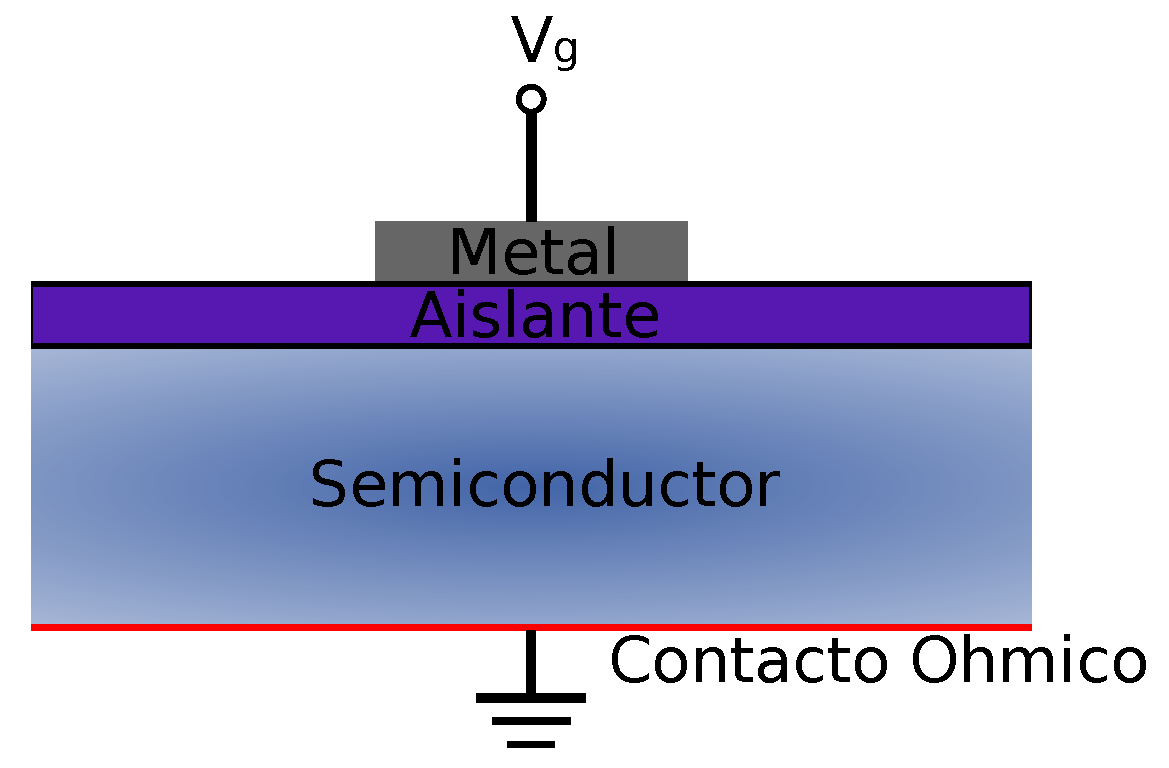
\includegraphics[scale=.35]{Figs/PixelCrossSection.pdf}
    \caption{\footnotesize{Esquema lateral de un capacitor MOS (píxel).}}
    \label{fig:PixelCrossSection}
\end{figure}
Además de los píxeles, como se puede ver en la Figura \ref{fig:ArgquitecturaCCDn}, los CCDs están compuestos de \textit{channel-stops} que se encargan de evitar que la carga de los píxeles migre entre columnas vecinas, mientras que los controladores verticales, con las señales $V_{1}$, $V_{2}$ y $V_{3}$, se encargan de desplazarla secuencialmente forma vertical. Otra parte fundamental de estos detectores es el registro horizontal, donde están los píxeles horizontales de la Figura \ref{fig:ArgquitecturaCCDn}, que es la región del CCD donde la carga es migrada de forma horizontal gracias a las fases $H_{1}$, $H_{2}$ y $H_{3}$ hacia el nodo de sensado.
\begin{figure}[h]
    \centering
        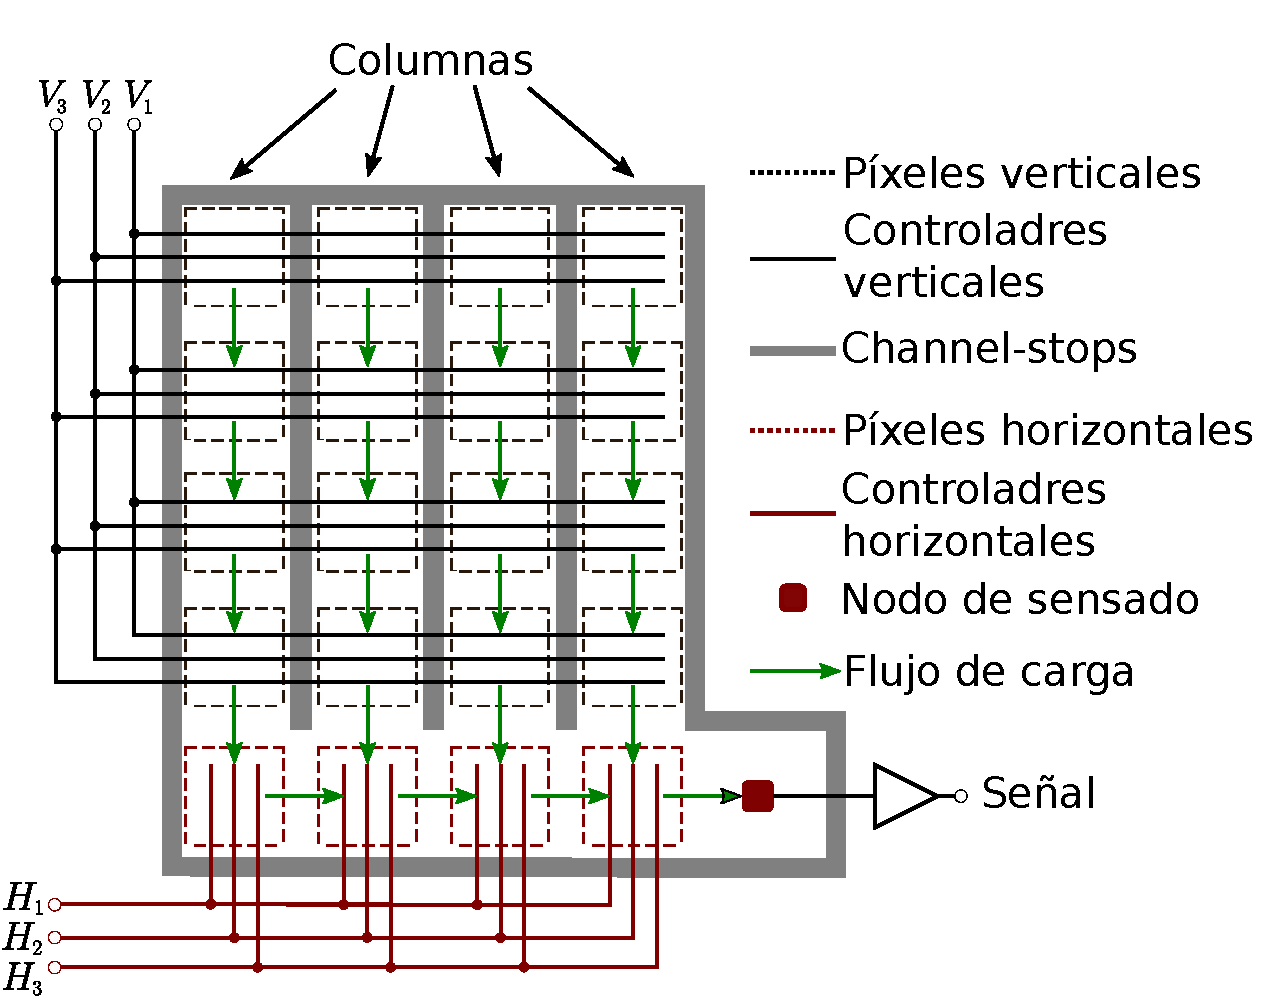
\includegraphics[scale=.5]{Figs/ArquitecturaCCD.pdf}
    \caption{\footnotesize{Ilustración esquemática de un sensor CCD de $4\times4$ píxeles. Las flechas muestran la dirección en la que la carga es desplazada para luego ser colectada por el nodo de sensado.}}
    \label{fig:ArgquitecturaCCDn}
\end{figure}
El principio de operación de un CCD se puede dividir en cuatro etapas, que a grandes rasgos son:
\begin{itemize}
    \item Exposición del detector: el tiempo de exposición es variable y depende del tipo de medición que se desee utilizar. Durante la exposición, la radiación incidente interactúa con el detector, generalmente generando pares electrón-hueco. 
    \item Colección: los electrones son luego arrastrados por el campo eléctrico del detector presente en su volumen hacia los pozos de potencial de los píxeles donde son colectados.
    \item Transferencia: dado que la medición de los píxeles se realiza de forma secuencial, la carga en cada uno de ellos debe ser transferida de un píxel a otro.
    \item Medición de la carga: a medida que se desplaza la carga, esta es llevada hacia el nodo de sensado donde finalmente es medida.
\end{itemize}
Los CCD's convencionales son capaces de alcanzar ruidos de lectura del orden de los $2\,e^{-}\si{rms/pix}$, gracias a la técnica de muestreo doblemente correlacionado\cite{Tiffenberg}. Sin embargo, en aplicaciones de bajas energías, el ruido electrónico de lectura presupone una barrera al límite de energías que pueden medirse con estos sensores para mantener la precisión deseada. Por debajo de los $2\,\si{keV}$ la contribución del ruido de lectura a la determinación de estas cantidades puede superar el $30\,\%$, como se esquematiza en la Figura \ref{fig:Fano_y_ruido}. La linea punteada representa el ruido constante de lectura presente en estos sensores y la recta representa un valor constante del factor de Fano para todo el rango de energías. Sobre la curva se ven los puntos que representan los valores del factor de Fano que se medirían si se utilizaran estos sensores debido a la suma de contribuciones del ruido sobre un factor de Fano constante de $0.1$.
\begin{figure}[H]
    \centering
        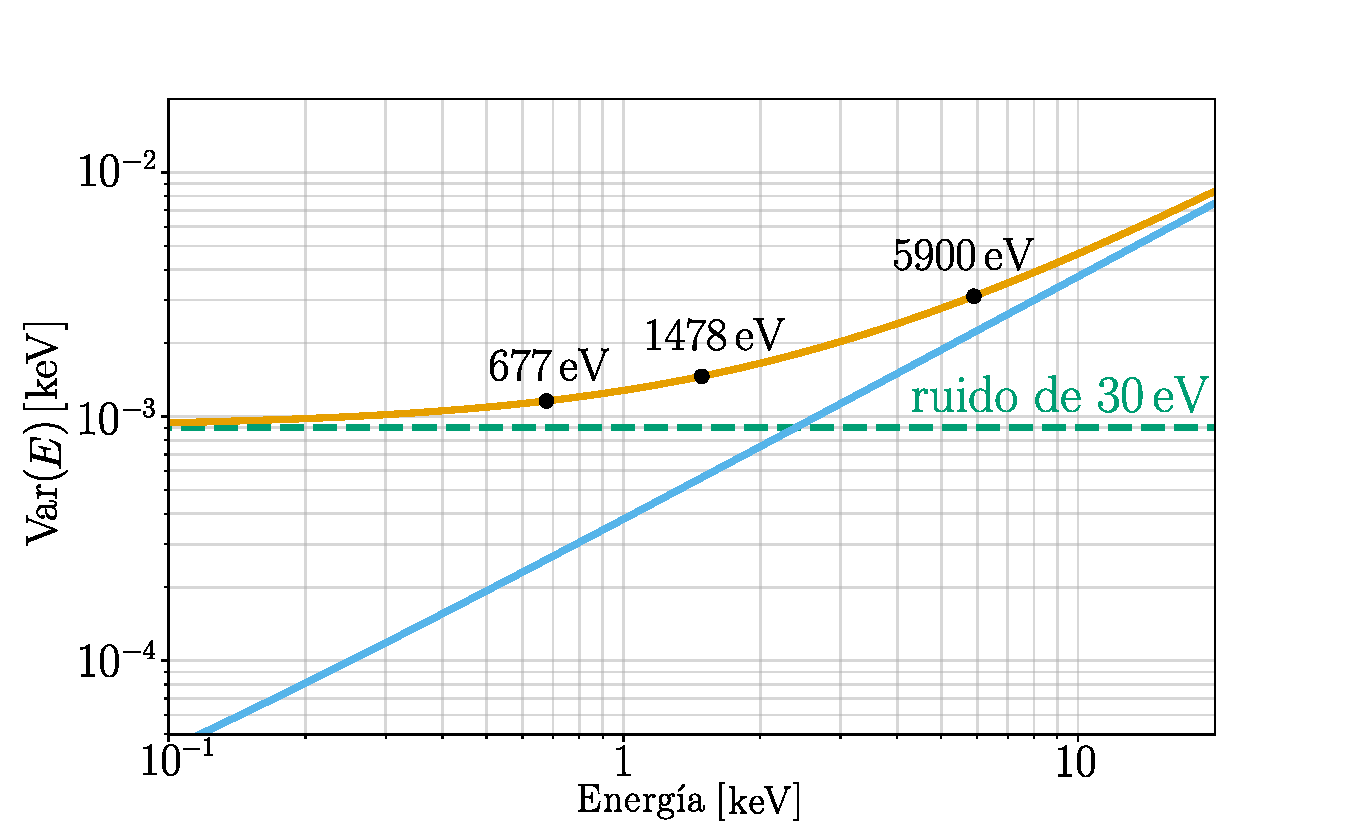
\includegraphics[scale=0.5]{Figs/fano_y_ruido.pdf}
    \caption{\footnotesize{Valores que ta se obtendrían de medir el factor de Fano con un sensor CCD convencional (puntos negros), debido a la contribución del ruido de lectura constante de $30\,\si{eV}$ (linea punteada horizontal). La linea recta continua representa un valor de factor de Fano constante.}}
    \label{fig:Fano_y_ruido}
\end{figure}
Los sensores \textit{Skipper}-CCD's, por otro lado, permiten disminuir el ruido electrónico de lectura a niveles subelectrónicos gracias a que son capaces de medir la carga en los píxeles de forma no destructiva. Esto permite tomar tantas mediciones como sean necesarias de la carga y estimar la carga real a partir de un promedio sobre el número de mediciones tomadas. Esta es la principal razón que motiva este trabajo, donde se realiza un estudio sistemático del factor de Fano a bajas energías, entre $1486\,\si{eV}$ (rayos X del Al) y $677\,\si{eV}$ (rayos X del flúor).
%%%%%%%%%%%%%%%%%%%%%%%%%%%%%%%%%%%%%%%%%%%%%%%%%%%%%%%%%%%%%%%%%%
%%%%%%%%%%%%%%%%%%%%%%%%%%%%%%%%%%%%%%%%%%%%%%%%%%%%%%%%%%%%%%%%%%
\section{Eficiencia de colección de carga y colección parcial de carga}
\noindent La Eficiencia de Colección de Carga o CCE (\textit{Charge Collection Efficiency}, por sus siglas en inglés) se define como la fracción del total de carga producida durante un evento de ionización que llega a la superficie del píxel del CCD y puede ser finalmente colectada durante el proceso de lectura. Para sensores del tipo \textit{fully depleted}-CCD\cite{osti_838066}, a los que se les aplican grandes potenciales, la CCE es aproximadamente del $100\,\%$, es decir, toda la carga producida por ionización en el volumen del sensor logra ser colectada y medida. Sin embargo, existen casos donde la eficiencia no alcanza el $100\,\%$ y esto es debido al fenómeno de Colección Parcial de Carga o PCC (\textit{Partial Charge Collection}, por sus siglas en inglés)\cite{PCC-CCE}. Este es un efecto que se debe a que en la región de los primeros micrones cercanos a la superficie contraria a la de colección de carga existe una probabilidad no nula de que la carga generada por ionización sufra recombinación, es decir, que vuelva a enlazarse a un átomo en vez de ser colectada por el píxel del sensor. Este efecto produce una disminución en el número de cargas que finalmente son llevadas a la superficie del sensor. En el esquema de la Figura \ref{fig:PCC} puede verse una vista en corte lateral de las primeras centenas de nanómetros de un CCD, donde debido al ángulo $\theta$ de incidencia de los rayos $X$ de la fuente, estos fotones generan cargas por ionización en la región donde hay recombinación. Una fracción de las cargas generadas $q_{i}$ logran ser colectadas, dependiendo de la profundidad del sensor donde se produjo la interacción. También se muestra que si la interacción se da fuera de esta región, toda la carga generada por ionización es colectada y $q_{i} = q_{f}$ y la eficiencia es máxima.
\begin{figure}%[H]
%Como reproducir este gráfico: correr el script NivelesOcupacionCarga.py ubicado en /Escritorio/Tesis2021/Figs/pys_para_plots y buscar la imagen en /home/igna/Escritorio/Tesis2021/Figs/
    \centering
        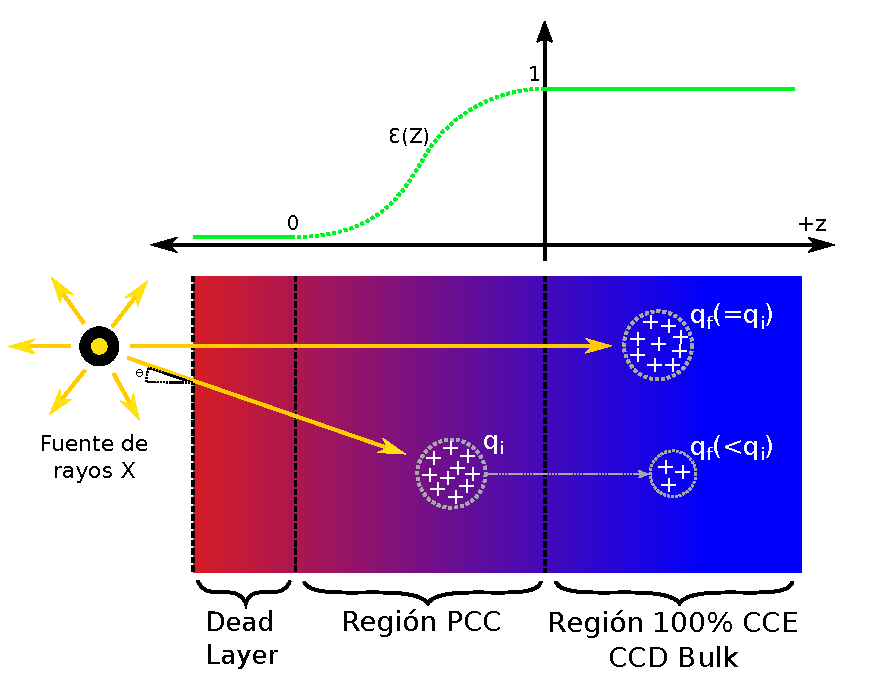
\includegraphics[scale=.8]{Figs/PCC.pdf}
    \caption{\footnotesize{Esquema lateral de las primeras centenas de nanómetros de un CCD, con una fuente de rayos $X$\cite{PCC-CCE}. Los fotones penetran en el sensor produciendo una nube de cargas $q_{i}$, de las cuales solo una fracción logra ser colectada. Esta aumentan monótonamente dependiendo de la profundidad de penetración.}}
    \label{fig:PCC}
\end{figure}
La colección parcial de carga es un problema propio de los sensores y de su fabricación. Sin embargo, existen tratamientos de la superficie posterior de estos sensores para reducir su impacto. Este es un proceso aplicado en CCDs para toma de imágenes astronómicas. 

El efecto que provoca la colección parcial de carga en las mediciones es el de agregar eventos con menor cantidad de carga de la que deberían, generando así colas a la izquierda de los picos de interés en los espectros y, por ende, agregando otro sesgo a la determinación de magnitudes dependientes del valor medio de los picos, como el factor de Fano.

%Por otro lado, la profundidad de la interacción depende del ángulo de incidencia y su distribución de probabilidad se puede escribir como
%\begin{equation*}
%    f_{Z}(z) = \frac{\cos{(\theta)}}{\lambda}e^{-z\frac{\cos{(\theta)}}{\lambda}}
%\end{equation*}
%donde $\lambda$ es la longitud de atenuación del fotón y depende de su longitud de onda. $\varepsilon(z)$ es la función \textit{eficiencia de colección de carga}
%\textcolor{red}{Reformulo lo anterior sin la dependencia con $\theta$}:


\section{Antecedentes \label{sec:Antecedentes}}
\noindent En trabajos previos se han estudiado las ventajas de la utilización de la tecnología \textit{Skipper} en los CCDs, para lograr medir con precisión subelectrónica en regímenes de energía donde los sensores CCD convencionales más precisos sólo podrían alcanzar resoluciones del orden de los $2$ electrones. Por primera vez fue usada para medir el factor de Fano y la energía de creación electrón-hueco en el silicio a una energía de $5.9\,\si{keV}$ a $123\,\si{K}$\cite{Rodrigues}.

Para lograr esto, se implementó un método de calibración absoluta que determinó la relación entre el número de electrones en cada píxel y la lectura del valor en ADUs (\textit{Analog Digital Unit} o Unidades analógico-digitales). El procedimiento para la calibración consistió en la utilización de un LED, que emitía fotones en $405\,\si{nm}$ de longitud de onda, para poblar los píxeles del sensor. Realizando un barrido en el tiempo de exposición del sensor a la luz del LED, se logró poblar a los píxeles del sensor con un amplio rango de cargas. La medición de carga se realizó tomando $300$ lecturas por cada píxel, gracias a la tecnología \textit{Skipper} que permite realizar múltiples muestreos de forma no destructiva, que luego fueron promediadas logrando reducir el ruido de lectura en un factor $\sqrt{300}$. Como resultado, se obtuvieron distribuciones de carga Gaussianas en los posibles niveles de ocupación de carga con una resolución tal que hizo posible distinguir perfectamente entre picos consecutivos, como se puede ver en la Figura \ref{fig:Calibracion}. De esta forma, mediante un ajuste gaussiano se pudo establecer el valor medio en ADUs para cada uno de estos picos, estableciendo como valor de carga el número de pico correspondiente. Así es que se obtuvo una relación uno a uno entre cantidad de carga por píxel y ADUs. Cabe destacar que para comenzar a numerar los picos, primero es necesario establecer el valor de $0$ carga o píxel vacío, lo cual no corresponde, a priori, a un valor nulo en ADUs. Para ello, las imágenes tomadas con \textit{Skipper} cuentan con una región denominada \textit{overscan} que se utiliza para calcular la linea de base y poder sustraerla luego a la carga de cada píxel, logrando así que la media de los píxeles vacíos quede en cero ADUs.
\begin{figure}[H]
%Como reproducir este gráfico: correr el script NivelesOcupacionCarga.py ubicado en /Escritorio/Tesis2021/Figs/pys_para_plots y buscar la imagen en /home/igna/Escritorio/Tesis2021/Figs/
    \centering
        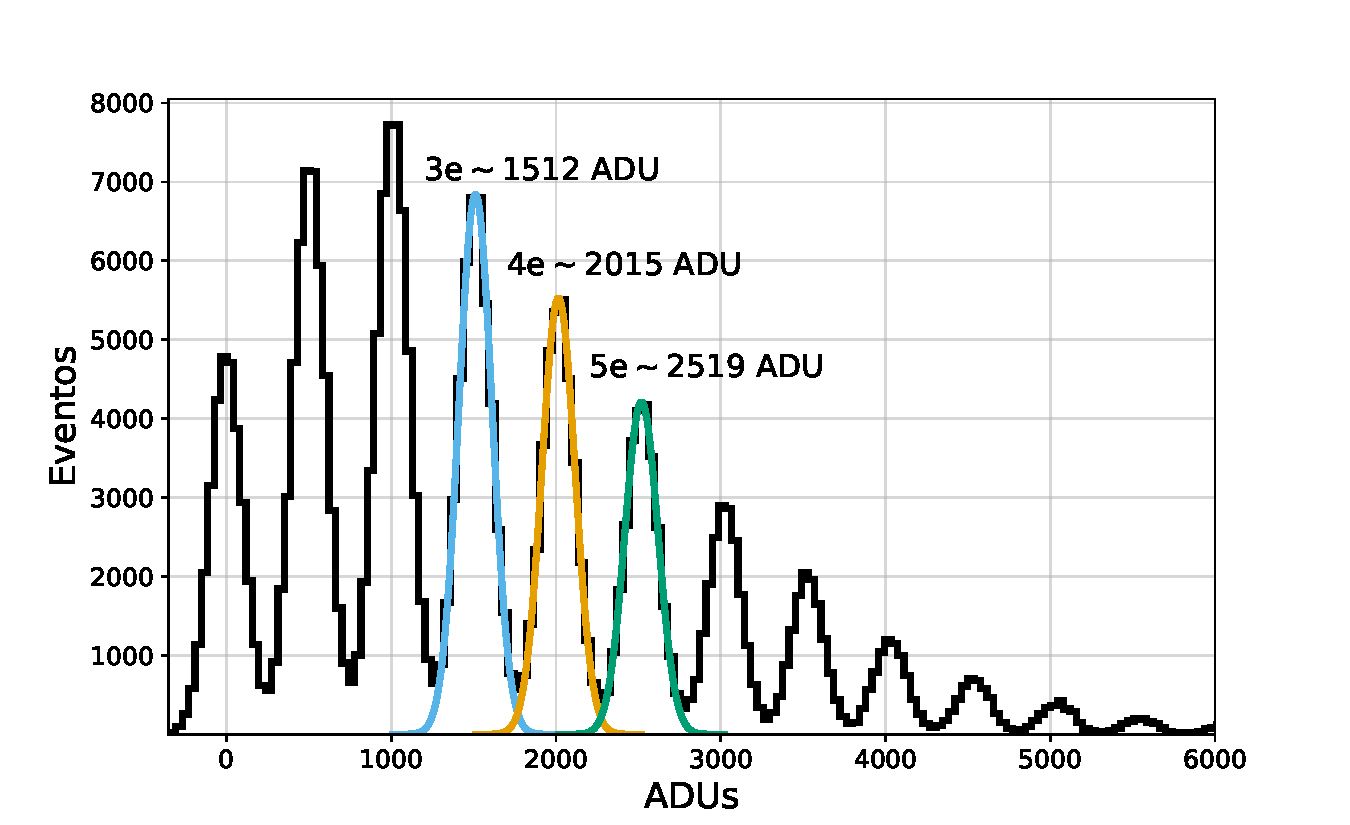
\includegraphics[scale=0.5]{Figs/ajuste_gaussiano_calibracion.pdf}
    \caption{\footnotesize{Histograma de los datos obtenidos al iluminar el CCD con LED, correspondiente a una región con poca ocupación, donde los picos de los ajustes entre electrones se distinguen a la perfección.}}
    \label{fig:Calibracion}
\end{figure}
Las mediciones del factor de Fano $F$ y la energía de creación electrón-hueco $\varepsilon_{\eh}$ se realizaron utilizando rayos $X$ de $5.9\,\si{\mbox{keV}}$ emitidos por una fuente de $\Fe{55}$. Más precisamente, rayos $X_{K}$, cuyas energías son las de la Tabla \ref{tab:EnergiasXk}.
\begin{table}[h]
\centering
\begin{tabular}{@{}ccc@{}}
\toprule
$X_{K}$         &   Energía [keV]   &   Intensidad relativa \\ \hline \hline
$\alpha_{2}$    &   $5887.6$        &   $8.5 (4)$           \\
$\alpha_{1}$    &   $5898.8$        &   $16.9 (8)$          \\
$\beta_{3}$     &   $6490.4$        &   $4.1 (11)$          \\ \bottomrule
\end{tabular}
\caption{\footnotesize{Energías e intensidades relativas de los fotones X emitidos tras el decaimiento de $\Fe{55}$}}
\label{tab:EnergiasXk}
\end{table}
Sobre los histogramas de los espectros obtenidos al irradiar el CCD con estos rayos $X$, se realizó un ajuste de los picos del espectro para obtener los parámetros $\mu$ y $\sigma$ de cada uno. Para esto, se utilizó la verosimilitud, cuya expresión es la de la ecuación \eqref{ec:verosimilitud}, que surge de la convolución de dos distribuciones exponenciales y una distribución gaussiana
{\small
\begin{align}
    \Lagr(e|\mu_{1},
            \mu_{2},
            \sigma_{1},
            \lambda_{1},
            \lambda_{2},
            \eta_{1} = \eta_{2},
            \eta_{3})
    = &
    \sum\limits_{j=1}^{3} I_{j}
    \left\{
        \eta_{j}\frac{\lambda_{1}}{2}
        \exp
            \left[
                (e-\mu_{j})\lambda_{1} + \frac{\sigma_{j}^{2}\lambda_{1}^{2}}{2}
            \right]
        \mbox{Erfc}
        \left[
            \frac{1}{\sqrt{2}}
            \left(
                \frac{e - \mu_{j}}{\sigma_{j}}
                +\sigma_{j}\lambda_{1}
            \right)
        \right] \right. \nonumber
        \\
        + &
        \left.
        (1-\eta_{j})\frac{\lambda_{2}}{2}
        \exp
            \left[
                 (e - \mu_{j})\lambda_{2}
                 + \frac{\sigma_{j}^{2}\lambda_{2}^{2}}{2}
            \right]
        \mbox{Erfc}
        \left[
            \frac{1}{\sqrt{2}}
            \left(
                \frac{e - \mu_{j}}{\sigma_{j}}
                +\sigma_{j}\lambda_{2}
            \right)
        \right]
    \right\}
        \label{ec:verosimilitud}
\end{align}
}%
donde $\mu_{j}$, $\sigma_{j}$ y $I_{j}$ representan el valor medio de carga, la desviación estándar del valor medio de carga y la intensidad relativa del pico $j$-ésimo con energía $E_{j}$, respectivamente y $j = \{\alpha_{1}, \alpha_{2}, \beta_{3}\}$. Además, $\lambda_{1}$ y $\lambda_{2}$ son parámetros de la distribuciones exponenciales y $\eta_{j}$ es el peso relativo entre ellas. La razón por la cual se utilizaron dos exponenciales y una gaussiana para modelar los picos, es porque se buscaba describir las colas que se generan a la izquierda de estos, de forma análoga a como describen en los picos en espectrometría alfa\cite{Bortels}. Sin embargo, se sabe que en este último caso, las colas no provienen del mismo fenómeno físico subyacente a los experimentos anteriormente mencionados.
%La Figura \ref{fig:AjusteNoBineado} representa el ajuste mediante la verosimilitud de los picos de rayos $X$ para un total de $18085$ eventos. Lo resultados para la medición del factor de Fano, la energía de creación electrón-hueco y demás parámetros relevantes se encuentran en la Tabla \ref{tab:ParametrosAjusteNoBineado}.
%\begin{figure}%[H]
%    \centering
%        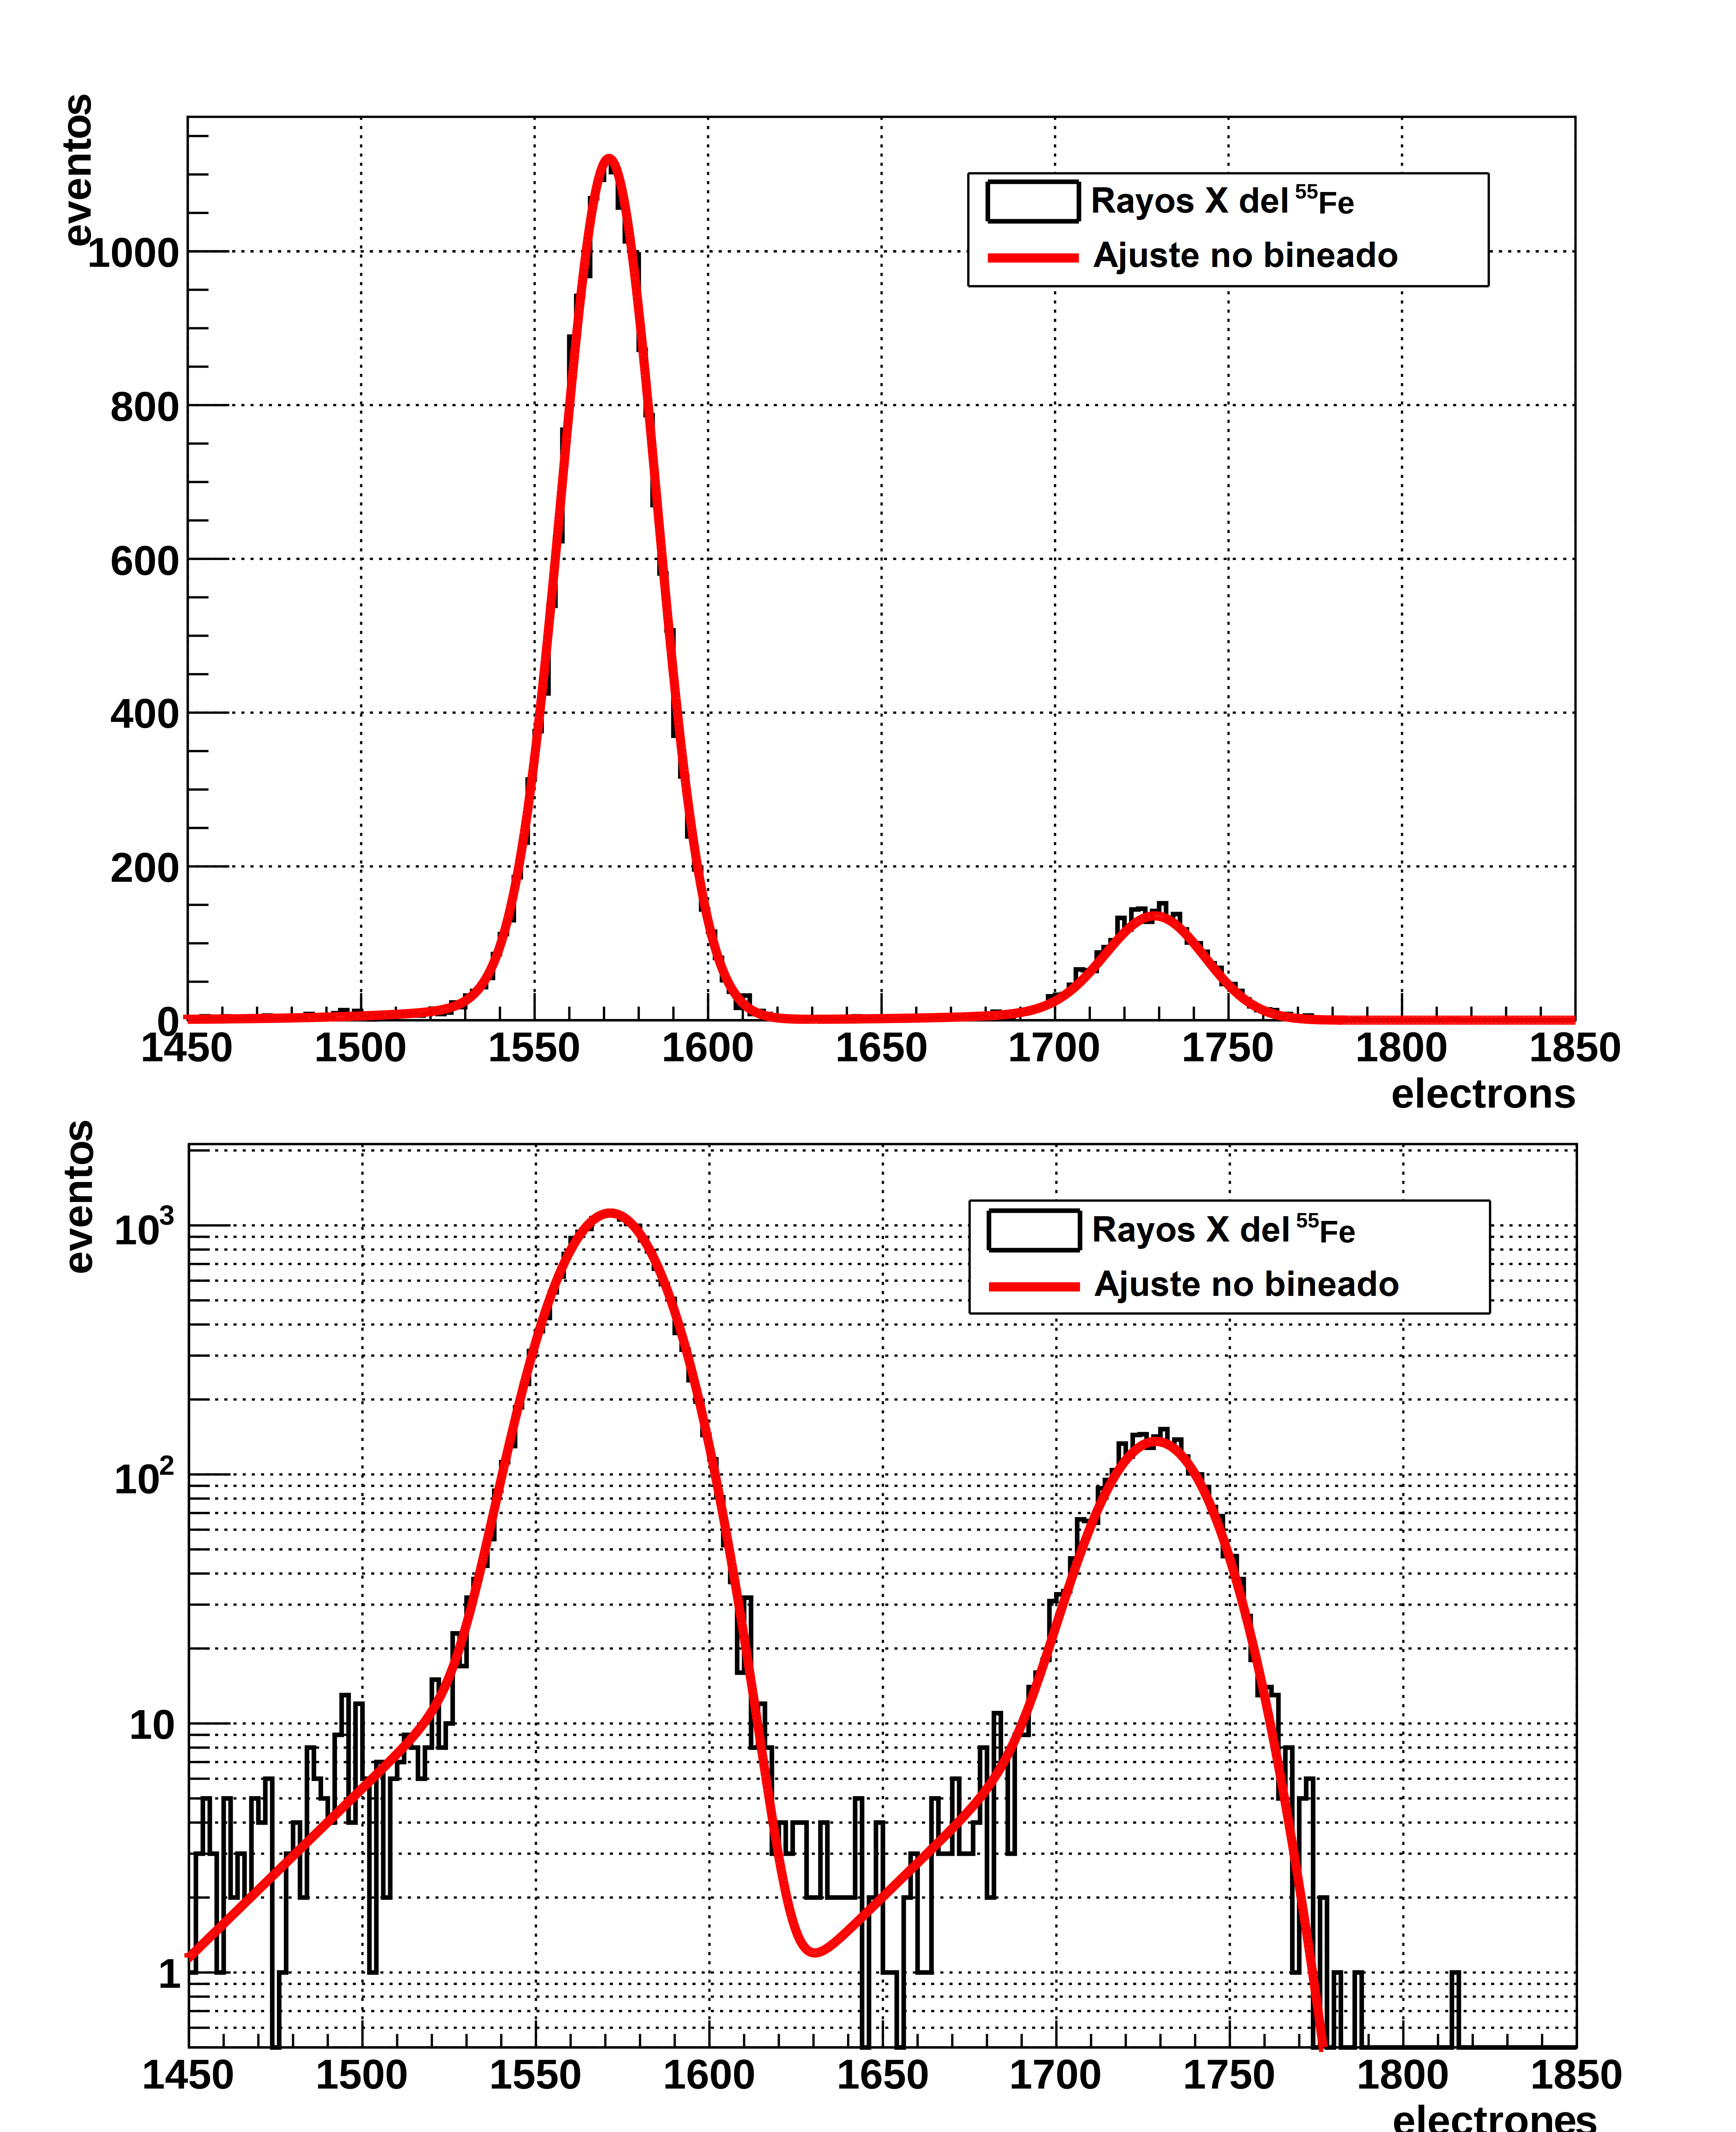
\includegraphics[scale=.15]{Figs/AjusteNoBineado.png}
%    \caption{\footnotesize{Ajuste no bineado de los picos de $\Fe{55}$.}}
%    \label{fig:AjusteNoBineado}
%\end{figure}
\begin{table}[h]
\centering
\begin{tabular*}{\textwidth}{c @{\extracolsep{\fill}} ccccccccc}%{@{}ccccccccc@{}}
\toprule
$X_{K}$ &
  $\mu\ [e^{-}]$ &
  $\Delta \mu\ [e^{-}]$ &
  $\sigma\ [e^{-}]$ &
  $\Delta \sigma\ [e^{-}]$ &
  $F$ &
  $\Delta F$ &
  $\varepsilon_{\eh}\ [\mbox{eV}/e^{-}]$ &
  $\Delta \varepsilon_{\eh} \ [\mbox{eV}/e^{-}]$ \\ \hline\hline
$\alpha_{2}$ &
  $1570.50$ &
  $0.18$ &
  $13.68$ &
  $0.12$ &
  \multirow{3}{*}{$0.119$} &
  \multirow{3}{*}{$0.002$} &
  \multirow{2}{*}{$3.749$} &
  \multirow{2}{*}{$0.001$} \\
$\alpha_{1}$ & $1573.48$ & $0.18$ & $13.69$ & $0.12$ &  &  &         &         \\
$\beta_{3}$  & $1730.50$ & $0.55$ & $14.36$ & $0.13$ &  &  & $3.751$ & $0.002$ \\ \bottomrule
\end{tabular*}
\caption{\footnotesize{Parámetros obtenidos de los ajustes para las mediciones del $\Fe{55}$. El factor de Fano se tomó el mismo para los tres picos y la energía de creación electrón hueco se fijó para que sea la misma en los picos $\alpha$.}}
\label{tab:ParametrosAjusteNoBineado}
\end{table}
Estos constituyen los primeros resultados obtenidos de la utilización de la tecnología \textit{Skipper}-CCD para el cálculo del factor de Fano y de la energía de creación electrón-hueco para una temperatura de $123\,\si{K}$ y se hallan condensados en la Tabla \ref{tab:ParametrosAjusteNoBineado}. Estos se encontraron en buen acuerdo con la bibliografía preexistente~\cite{Ryan, Alig, Kotov}.

Además, se avanzó en las primeras mediciones del factor de Fano y la energía de creación electrón-hueco para energías por debajo de los de $2\,\si{keV}$~\cite{TesisKevin}, más específicamente, para energías de $677\,\si{eV}$ y $1486\,\si{eV}$, que corresponden a los rayos $X$ de fluorescencia del flúor y del aluminio respectivamente. En la Tabla \ref{tab:EnergiasFluorescenciaFAl} pueden verse las energías e intensidades relativas para los rayos $X$ de estos elementos. En este caso, utilizando toda la maquinaria desarrollada para el $\Fe{55}$, se realizaron mediciones con una fuente de $\Am{241}$ que emite partículas alfa con una energía de $\sim 5.6\,\si{MeV}$. A estas partículas luego se las hizo impactar contra una cinta de teflón y una barra de aluminio que por fluorescencia emitían rayos $X$ con las energías antes mencionadas. Cabe destacar que se trató de evitar que las partículas alfa alcanzaran el detector, dado que son partículas muy energéticas y por tanto no son eventos de interés.
\begin{table}[h]
\centering
\begin{tabular}{@{}cccc@{}}
\toprule
Elemento    &   $X_{K}$         &   Energía [eV]    &   Intensidad relativa \\ \hline \hline
F           &   $\alpha_{1,2}$  &   $676.8$         &   $148$               \\
Al          &   $\alpha_{2}$    &   $1486.3$        &   $50$                \\
Al          &   $\alpha_{1}$    &   $1486.7$        &   $100$               \\
Al          &   $\beta_{1}$     &   $1557.4$        &   $1$                 \\ \bottomrule
\end{tabular}
\caption{\footnotesize{Energías e intensidades de las lineas de emisión de rayos $X$ para el flúor y el aluminio en el rango de energías por debajo de los $2\,\si{keV}$.}}
\label{tab:EnergiasFluorescenciaFAl}
\end{table}

Uno de los desafíos que surgieron en este otro trabajo fue que solo una fracción de los átomos que son impactados por las partículas alfa se desexcitan emitiendo fotones $X$ en las energías de interés. Es por esto que la tasa de eventos medidos es considerablemente menor en comparación a la que se obtuvo al medir con la fuente de $\Fe{55}$.

Con los datos de estas mediciones se reconstruyeron los espectros para ambos picos y se les realizó un ajuste no bineado, similar al utilizado en los experimentos con $\Fe{55}$, utilizando la verosimilitud descripta por la expresión \eqref{ec:verosimilitudF-Al}.
\begin{align}
    \Lagr(e|\mu,
            \sigma,
            \lambda_{1},
            \lambda_{2},
            \eta)
    = &
    \eta
    \left\{
        \frac{\lambda_{1}}{2}
        \exp\left[
                (e-\mu)\lambda_{1} + \frac{\sigma^{2}\lambda_{1}^{2}}{2}
            \right]
        \mbox{Erfc}
        \left[
            \frac{1}{\sqrt{2}}
            \left(
                \frac{e - \mu}{\sigma}
                +\sigma\lambda_{1}
            \right)
        \right] \right\} \nonumber
        \\
        + &
        (1-\eta)
        \left\{
        \frac{\lambda_{2}}{2}
        \exp
            \left[
                 (e - \mu)\lambda_{2}
                 + \frac{\sigma^{2}\lambda_{2}^{2}}{2}
            \right]
        \mbox{Erfc}
        \left[
            \frac{1}{\sqrt{2}}
            \left(
                \frac{e - \mu}{\sigma}
                +\sigma\lambda_{2}
            \right)
        \right]
    \right\}
        \label{ec:verosimilitudF-Al}
\end{align}
En este caso, el ajuste resultó mucho más sensible a los cambios en el bineado del histograma, debido a que la tasa de eventos registrados para este experimento fue mucho menor. Los resultados obtenidos en este trabajo a partir de los ajustes de estas mediciones se encuentran en la Tabla \ref{tab:ParametrosAjusteNoBineadoF-Al}.
\begin{table}[h]
\centering
\begin{tabular*}{\textwidth}{c @{\extracolsep{\fill}} ccccccccc}%{@{}ccccccccc@{}}
\toprule
Elemento&
  $\mu\ [e^{-}]$ &
  $\Delta \mu\ [e^{-}]$ &
  $\sigma\ [e^{-}]$ &
  $\Delta \sigma\ [e^{-}]$ &
  $F$ &
  $\Delta F$ &
  $\varepsilon_{\eh}\ [\mbox{eV}/e^{-}]$ &
  $\Delta \varepsilon_{\eh} \ [\mbox{eV}/e^{-}]$ \\ \hline\hline
  F &   $182.0$ &   $0.8$  &   $7.0$   &   $0.7$   &   $0.27$  &   $0.05$  &   $3.72$ &   $0.02$\\
  Al&   $404.4$ &   $0.4$  &   $8.3$   &   $0.3$   &   $0.17$  &   $0.01$  &   $3.679$ &   $0.004$\\ \bottomrule
\end{tabular*}
\caption{\footnotesize{Resultados preliminares obtenidos en trabajos previos para el factor de Fano y la energía de creación electrón-hueco para los rayos $X$ del flúor y el aluminio.}}
\label{tab:ParametrosAjusteNoBineadoF-Al}
\end{table}

Sin embargo, estos últimos son resultados preliminares y pueden mejorarse tanto las mediciones como el tratamiento de datos. Además, los ajustes utilizados hasta el momento no provienen en su totalidad de modelos representativos de la física subyacente al proceso de generación de carga por ionización y los efectos que la colección parcial de carga produce sobre ella. Puede decirse que estos modelos son \textit{ad hoc}, sin embargo resultaron de gran utilidad para realizar los ajustes previamente.

Es a partir de aquí donde este trabajo continua con el estudio del factor de Fano, la energía de creación electrón hueco y el fondo presente en las imágenes para el rango de energías por debajo de los $2\,\si{keV}$.

%%%%%%%%%%%%%%%%%%%%%%%%%%%%%%%%%%%%%%%%%%%%%%%%%%%%%%%%%%%%%%%%%%
%%%%%%%%%%%%%%%%%%%%%%%%%%%%%%%%%%%%%%%%%%%%%%%%%%%%%%%%%%%%%%%%%%
\section{Motivación del análisis de imágenes}
\noindent El fondo presente en las imágenes tiene diferentes orígenes, uno de ellos es la carga producida por fluctuaciones térmicas en la red cristalina del silicio del sensor (corrientes oscuras). Otra contribución es la de eventos de dispersión Compton, producidos por la interacción de los fotones con los materiales que rodean al sensor, y también en la red cristalina del mismo. Podemos incluir además, aquellos fotones infrarrojos emitidos desde los materiales que rodean al detector cuando estos son excitados por radiación circundante. También se encuentran los eventos de carga producida por radiación muy penetrantes provenientes del exterior, como por ejemplo, muones.

El análisis consistió en estudiar el efecto que produce el fondo de las imágenes sobre los eventos de interés: la aglomeración de píxeles con un único electrón alrededor de los clusters, y la carga extra añadida sobre ellos. En muchos casos resulta que los píxeles con fondo se aglutinan a los clusters, aumentando su tamaño y su carga, o incluso también haciendo de puente entre dos clusters vecinos. Estos son dos efectos indeseados, primero porque sesga la cantidad de carga real en un evento de interés y segundo porque los programas de reconocimiento de eventos podrían %
%el algoritmo de clusterización podría %
ignorarlos al no cumplir con los cortes de calidad impuestos, tanto por forma como por cantidad de carga, produciendo así una disminución en la estadística.

Es entonces necesario utilizar un umbral de detección que ignore estos píxeles con carga menor a dos electrones, de forma de evitar el aglutinamiento de píxeles con fondo a los clusters de interés y así aumentar la estadística en el conteo de eventos. Pero también es necesario lograr caracterizar este fondo para corregir el sesgo introducido por el nuevo umbral de detección, el cual, también eliminará píxeles con carga genuina. Es por eso que en este trabajo se propuso un análisis de las imágenes que pueda determinar el umbral más conveniente a utilizar y recuperar la mayor cantidad de estadística posible, además de un método para estimar en valores medios cuántos eventos genuinos son removidos y cuántos eventos espurios hay en los clusters, para mejorar así las incertezas en la determinación del factor de Fano y la energía de creación electrón-hueco a bajas energías.
%%%%%%%%%%%%%%%%%%%%%%%%%%%%%%%%%%%%%%%%%%%%%%%%%%%%%%%%%%%%%%%%%%
%%%%%%%%%%%%%%%%%%%%%%%%%%%%%%%%%%%%%%%%%%%%%%%%%%%%%%%%%%%%%%%%%%
\section{Organización de la tesis}
\noindent En el presente capítulo se ha dado una breve introducción a los 3 aspectos principales de estudio de este trabajo: El factor de Fano, la energía de creación electrón hueco y la colección parcial de carga. Además se han presentado resultados que conforman los antecedentes para la motivación de este trabajo

En el capítulo \ref{chap:simulaciones} se presenta un modelo físico simple de la interacción entre fotones incidentes y la red del sensor, que luego es estudiado a partir de simulaciones Monte Carlo.

En el capítulo \ref{chap:ConfiguracionExperimental} se desarrolla una descripción esquemática del dispositivo de medición utilizado, los regímenes de trabajo necesarios para realizar las mediciones. También se halla una breve descripción del sensor y de los materiales que lo componen, como así también de la fuente radioactiva utilizada. Por último, se describe el proceso de medición.

En el capítulo \ref{chap:Analisis} se describe como son procesados los datos y qué programas son utilizados además de las pruebas realizadas con distintos umbrales. También se muestran diferentes análisis de caracterización del sensor y sus diferentes cuadrantes. Es en este capitulo que se describen los diferentes enfoques utilizados en la estimación del fondo y de la cantidad de eventos eliminados por el umbral y el método aplicado para realizar las correcciones sobre la carga.

En el capítulo \ref{chap:ModeloPCC} se introduce un novedoso modelo de ajuste para los picos de los histogramas, que tiene en cuenta el fenómeno de colección parcial de carga.

Por último, en el capítulo \ref{chap:Resultados} se presentan los resultados obtenidos a partir de estos análisis y las perspectivas a futuro.


%%%%%%%%%%%%%%%%%%%%%%%%%%%%%%%%%%%%%%%%%%%%%%%%%%%%%%%%%%%%%%%%%%
%%%%%%%%%%%%%%%%%%%%%%%%%%%%%%%%%%%%%%%%%%%%%%%%%%%%%%%%%%%%%%%%%%
%%%%%%%%%%%%%%%%%%%%%%%%%%%%%%%%%%%%%%%%%%%%%%%%%%%%%%%%%%%%%%%%%%